\documentclass[11pt]{report}
\usepackage[spanish]{babel}
\usepackage[utf8]{inputenc}
\usepackage{graphicx}
\usepackage{geometry}
\usepackage{fancyhdr}
\usepackage{amsmath}
\usepackage{helvet}
\usepackage{titlesec}
\usepackage{setspace}
\usepackage{tocloft}
\usepackage{hyperref}
\usepackage{csquotes}
\usepackage{placeins}
\usepackage{comment}

\setlength{\parskip}{0.5em}

\usepackage[style=numeric,sorting=none]{biblatex}
\addbibresource{referencias.bib} 

\onehalfspacing
\renewcommand{\familydefault}{\sfdefault}

\geometry{
  letterpaper,
  left=3cm,
  right=2cm,
  top=2.5cm,
  bottom=2cm,
}

\addto\captionsspanish{
  \renewcommand{\contentsname}{Índice}
}
\renewcommand{\cftchapdotsep}{\cftdotsep}  % Para capítulos
\renewcommand{\cftsecdotsep}{\cftdotsep}   % Para secciones
\renewcommand{\cftsubsecdotsep}{\cftdotsep} % Para subsections

\titleformat{\chapter}[display]
  {\normalfont\Large\bfseries}
  {\chaptername\ \thechapter}
  {10pt}
  {\huge}
\titlespacing*{\chapter}{0pt}{-20pt}{20pt}  % Ajusta el espaciado aquí

\begin{document}

Cuando se habla de motores eléctricos de corriente continua, los motores sin escobillas resaltan por su alto desempeño, siendo la opción obligatoria cuando se trata de autos eléctricos, drones, robótica avanzada y robótica industrial.

%estos motores se parten con el diseño de Nikola Tesla en 1888, del primer motor de corriente alterna sincrono

%por ejemplo el robot cheetah del MIT
%los motores paso a paso utilizados en robots industriales también son un tipo de motor brushless
%todos los autos eléctricos utilizan motores sin escobillas
%la categoría eléctrica de formula 1 utiliza brushless
%solo los drones de baja categoría utilizan motores brushed
%los scooters eléctricos también utilizan brushless

%esto es debido a algunos aspectos como su mayor densidad de potencia, que permite hacer robots mas livianos, al no tener escobillas ni partes con rozamiento ademas de los rodamientos, estos motores requieren poco mantenimiento y su vida util es mayor.

Para los motores brushless, existe una gran diversidad de técnicas de control. Algunas de las más relevantes son el control trapezoidal, mayormente utilizado en drones, el control directo de torque (DTC), que se usa principalmente en motores de media-alta potencia, y el control FOC, que es mayormente utilizado en robótica. En este documento, solo se hablará de esta última técnica.

Hay tres aspectos que diferencian cada técnica. Estos son el rizado de torque, el coste computacional y la complejidad del hardware necesario para su ejecución. En estos aspectos, el control FOC es uno de los que produce menor rizado de torque, pero requiere de una mayor cantidad de computación y hardware.

Este proyecto presenta la implementación y validación de un controlador de campo orientado (FOC) para motores sin escobillas de corriente continua (BLDC). Se desarrolló la placa controladora utilizando STM32 y se implementó el algoritmo del control FOC en C.


\chapter*{Marco teórico}
\addcontentsline{toc}{chapter}{Marco teorico}

\section{Motores brushless}
Los motores brushless (BLDC) o motores sin escobillas de corriente continua son motores donde el embobinado del motor se encuentra en el estátor, mientras que el rotor tiene los imanes.

Estos motores se caracterizan por su mayor densidad de potencia en comparación con los motores con escobillas. Sin embargo, esto también lleva a una mayor complejidad al requerir un controlador que realice la conmutación del embobinado para generar el giro del rotor.

%estos motores pueden tener configuraciones monofasicas, bifasicas y trifasicas, aun que para este proyecto, solo se van a abarcar los motores en configuración trifasica

Al tener tres fases que se pueden energizar de forma positiva o negativa, esto da ocho posibles configuraciones de polarización, de las cuales dos son nulas, dando así seis formas de polarización útiles para el control del giro. Esto es lo que da origen a uno de los métodos de control más simples, que es el control trapezoidal o control de seis pasos, que simplemente se limita a ejecutar estas seis polarizaciones en secuencia para completar un giro, pero sacrificando eficiencia y agregando un rizado en el torque bastante importante.

%los motores BLDC suelen ser utilizados siempre que se habla de robótica avanzada, gracias a su gran versatilidad, densidad de potencia y capacidades para realizar un control preciso de su velocidad, posición y torque,


\section{Motivación}
%\addcontentsline{toc}{chapter}{Motivacion}
%En robótica, siempre que se habla de robots avanzados y de alto desempeño, entra en tema el uso de motores brushless y en estos motores, el control mas utilizado es el control FOC,
%En los robots sumo para la ALL JAPAN ROBOT SUMO TOURNAMENT suelen utilizar motores brushed de la marca Maxon, dejando de lado a los motores brushless, ya que al controlarlos con un ESC con control trapezoidal y ademas en motores sin sensor, estos motores no tienen torque para el arranque
%en las competencias de robot sumo, un aspecto Fundamental es tener alto torque y gran estabilidad en el control

%el motivo fundamental es hacer la implementación para su uso en robots sumo y como extra también para utilizar en seguidores de linea
%con la idea de tener un controlador compacto, liviano y de alto desempeño, aun si su eficiencia es baja, con algún protocolo que permita una comunicación rápida y sencilla, para asi poder agregar controladores externos
%para esto, se necesita un controlador diseñado para un uso altamente intenso y de corta duración, llegando a sobre cargar el motor hasta sus limites nominales
%los drivers comerciales que se puedes adquirir de forma sencilla o son muy grandes y pesados o solo pueden trabajar con el motor dentro de su rango nominal
%ademas ningún controlador tiene capacidad para utilizar técnicas de fortalecimiento y debilitamiento del campo electromagnético de forma activa para poder sobre pasar los rangos nominales

Este proyecto nace de la necesidad de un controlador para motores brushless adecuado para su uso en robots de competencia en la categoría de robot sumo autónomo. En esta categoría, este tipo de motores no son normalmente utilizados debido a las limitaciones de los controladores comerciales y los riesgos que conlleva la sobrecarga de los motores en periodos cortos de acción, ya que los controladores comerciales no están pensados para esto.

%en esta categoría debido a las limitaciones de peso y dimensiones, el tener un motor que pueda entregar una gran potencia en lapsos cortos de tiempo se vuelve fundamental, esto ya esta logrado en motores con escobillas, donde los competidores dan un sobre voltaje al motor y utilizan controladores de mas corriente de la nominal de motor, para asi poder obtener un extra de desempeño del motor, sin tener que recurrir a motores mas grandes aun si esto sacrifica la eficiencia y acorta la vida util del motor

%en este aspecto, los motores brushless, gracias a su mayor densidad de potencia, debería de poder ofrecer un desempeño mas adecuado para esta categoría, pero esta la limitación de que no existen controladores pensados para este propósito

%\addcontentsline{toc}{chapter}{Alcances}
\begin{comment}
\begin{itemize}
	\item Configurar el microcontrolador con STM32CubeMX.
	\item Implementar el controlador de velocidad y corriente.
	\item No se va a implementar el control de posición.
	\item Se va a programar el firmware utilizando VScode y C.
	\item Se compilará el firmware con makefile y GCC con la extensión STM32 por VScode.
	\item Cargar el firmware con STM32CubeProgrammer y ST-link.
	\item Diseñar la PCB en Eagle.
	\item Diseñar piezas extra en Autodesk Inventor y posterior fabricación en impresión 3D.
	\item Fabricar y semi ensamblar la PCB con JLCPCB.
	\item Obtener datos detallados en tiempo de ejecución.
	\item Graficar los datos con Plotly en Python.
	\item Identificar posibles mejoras.
\end{itemize}
\end{comment}

%--------------------
%Hardware

%en cuanto a hardware se intento mantener una placa solo con lo mínimo y necesario para la ejecución del control FOC, se utilizo en microcontrolador STM32H743VIT6
%se considero el agrear pines en las señales de control con el fin de poder conectar un analizador lógico y poder realizar un debug de estas
%al las señales de control del puente mosfet se le agregaron compuertas AND, para agregar la señal EN_GATE
%se utilizo un USB C, en configuración de USB 1.1, con posibilidad de alimentar la electronica de control, pudiendo desconectarlo con un jumper
%ademas de los botones de reset y boot del microcontrolador se dejaron 3 botones de propósito general
%se dejaron algunos leds para indicaciones de estado
%como el propósito de esta placa es cumplir el rol de placa de desarrollo, se dejaron disponibles todos los GPIO que no se llegaron a utilizar en una regleta
%también se agrego un puerto SPI, para poder en algún futuro experimentar con encoders obsoletos

%en cuanto a componentes, se utilizo un controlador de puerta UCC27211, que es también utilizado en Vesc, ya que es un buen compromiso entre circuito sencillo con un alto desempeño, pudiendo trabajar con mosfet mas grandes que el controlador DRV8301 utilizado en Odrive

%en cuanto a mosfet se utilizo el BSC011N03LSI, principalmente por disponibilidad para su ensamble en JLCPCB, ofrece buenas características a un bajo precio, con la posibilidad de poder ser mejorado, al haber mosfet de mayor rendimiento en el mismo encapsulado 

%para el sensor de corriente se utilizaron 2 resistencias de 1mOhm en paralelo, con un amplificador INA240A1, que tiene una ganancia de 20 V/V, para cada fase, este integrado y configuración también se tomo desde el diseño de Vesc, ademas de estar disponible para ensamblaje en JLCPCB, aun que el valor de las resistencias se ajusto considerando los rangos de corriente que deberán de soportar los mosfet y la potencia de disipación maxima que soportan las resistencias

%la selección de todos los GPIO para cada parte del driver se seleccionaron primero por su disponibilidad en la configuración del microcontrolador con cubeMX y también por la facilidad para rutear en la PCB

%no se utilizaron simulaciones para verificar el diseño y ruteo de la PCB

%para el reloj del microcontrolador se utilizo un cristal de 25Mhz en el puerto HSE del microcontrolador

%---------------
%Software

%con cubeMX se realiza toda la configuración del microcontrolador, relojes, periféricos,interrupciones, permisos de las regiones de memoria, etc.
%esta configuración se genera para funcionar con makefile
%esto genera un archivos makefile con las dependencias básicas que requiere el compilador, cualquier extra debe ser agregado
%cubeMX ademas genera todas las librerías HAL, aun que solo agregas las mínimamente necesarias al makefile
%cubeMX también genera un archivo linker de memoria, que debe ser modificado para utilizar el DMA
%desde VScode con la extension "STM32 for VScode" y sus dependencias se puede compilar el código con GCC 
%esta extension crea el archivo "STM32-for-VSCode.config.yaml" a partir del makefile generado por cubeMX
%todas las librerías y modificaciones que se agregan para la compilación se deben agregar en este archivos
%la librería genera un nuevo archivo de makefile a partir de este .yaml con el cual realiza la compilación del proyecto
%con simplicidad para instalar las dependencias del entorno de desarrollo, se utilizo un ubuntu ejecutado desde un WSL en windows
%esto permite tener un terminal de Linux desde el cual me puedo conectar con VScode para programar y luego puedo tomar el compilado para cargarlo al microcontrolador con STM32CubeProgrammer y el programador ST-LINK
%toda la programación en C se intento dividir en varias librerías para cada función del código
%ademas de utilizar estructuras para juntar las variables de cada funcionalidad
%no se utilizo C++ ya que todas las funciones de las librerías HAL están en C y requiere algunas consideraciones extra para poder programar el microcontrolador con C++, es posible, pero por mantener la programación algo mas sencilla, se prefirió mantener la programación en C

%en la placa controladora se dejaron 3 botones de acción, estos se utilizan para llevar el motor al home, activar el control de motor, desactivar el control de motor y empezar la captura de datos

%el controlador del motor se ejecuta en la interrupción del timer principal del motor, el cual también se encarga de las señales PWM para el puente mosfet, estas interrupciones se ejecutan a 48khz, con un reloj base del timer de 240MHz
%la interrupción parte con una lectura e interpretación de todos los sensores, como la lectura de los analógicos, obtención del contador del encoder y demás para después ejecutar el control del motor que se basa en una maquina de estados
%esta maquina de estados utiliza internamente una pila circular para la gestión de las tareas y cambios de estados

%para la lectura de los analógicos se configuraron los ADCs en dos formas
%para los sensores de corriente se utilizo el ADC 1 con una configuración de lectura inyectada que es activada por el timer 15, el cual va sincronizado con el timer 1, pero genera una señal de salida algunos ciclos antes de la ejecución de la interrupción del timer 1, esto con el fin de que las lecturas del ADC se sincronicen con el centro de la señal PWM en el puente mosfet ademas de permitir que estén ya disponibles al momento de obtener su valor en la interrupción principal
%para el sensor del voltaje de bus se utilizo el ADC 3, el cual esta configurado con una conversion normal que se ejecuta de forma continua y asincronica con el timer 1, utilizando el DMA para transferir los valores de la lectura a la memoria para su obtención en cualquier momento
%ademas se utilizo el ADC 2 para la lectura de 3 potenciómetros con los cuales se controla el motor, dependiendo de la modalidad de control que se quiera empelar, este ADC al igual que el ADC 3 utiliza una conversion continua y el DMA

%para el encoder se utilizo un encoder incremental un index (ABI), para las señales AB, se utilizo en timer 3 que es de 16 bits en modo encoder, lo cual permite hacer una gestión de estas señales por hardware, para el cual después simplemente se obtiene el valor del contador del timer 3, agregando si una gestión para el desbordamiento del contador, expandiendo la capacidad del contador de los 16bits por hardware a 64bits de forma virtual, prolongando el tiempo que este registro puede funcionar de forma continua
%ademas para tener una gestión precisa de los tiempos se utilizo el timer 2, que es un timer de 32bits, con un reloj de 240MHz, junto a una gestion de su desbordamiento
%este timer se utiliza para detectar la señal del index, lo que me permite saber el momento exacta en el cual ocurrió la señal
%ademas entre las señales A y B del encoder se agrego una compuerta XOR, esto genera una señal X4 del encoder, la cual se lee con el timer 2 para tener una referencia exacta de los tiempos entre señales del encoder
%esto es principalmente para no limitar la medición del tiempo en el encoder a múltiplos del periodo de las interrupciones y asi tener mediciones mas exactas de velocidad y aceleración

%para el código de obtención de datos o mal llamado en el código como debug, se utilizo una pila circular que ocupa una de las regiones de memoria ram del microcontrolador para almacenar los valores de las variables del sistema al final de cada interrupción para posteriormente ser enviados por el USB paquetes binario, estos datos son recepcionados en un código python que desempaqueta cada mensaje y va almacenando los valores en un CSV
%estos datos en los archivos CSV son graficados posteriormente con plotly con otro código python 

%em código para empezar el control de motor primero realiza una activación del puente mosfet, que consiste en primero activar las señales PWM del timer dejando un pequeño lapso para su estabilización y posteriormente activando las señales a los controladores de puerta con el pin EN_GATE

%ya que el algoritmo de FOC requiere la obtención de valores seno y coseno en sus transformadas y la ejecución de estas funciones son costosas en cuanto a tiempo de ejecución, se utilizo la librería CMSIS DSP, que se puede agregar en cubeMX, esta librería ya incorpora las funciones para estimar los valores seno y coseno a partir de tablas pre calculadas, optimizando su rendimiento para procesadores ARM

\begin{comment}
\section{Validación adquisición de Corriente}
%El sensor de corrientes se basa en resistencias shunt de valor conocido que se ubican en las fases del motor a la salida de los mosfet, el voltaje de caída en esta resistencia es amplificada por un amplificador de instrumentación INA240A1 con una ganancia de 20V/V y posteriormente adquirido por el ADC1 del microcontrolador que cuenta con una resolución de 16bits.

%En el INA240A1 aplica un offset en el voltaje de salida que corresponde a la mitad del fondo de escala.

%Una ves adquiridos los datos, en el microcontrolador se resta el offset y se escala para su uso en valores de amperios.

%La medición de corriente se realiza solo en las fases A y B, mientras que la fase C se estima asumiendo que el sistema es un sistema trifásico equilibrado.

%Posteriormente al escalado de las corrientes de fase, estos son utilizados para los cálculos de la transformada Clarke y transformada Park.

%A estas señales se les aplica un filtro complementario ajustado para tener una frecuencia de corte de 12000hz para las corrientes de fase y 800hz para las corrientes directa y cuadratura.

Se validara el funcionamiento y adquisición de las mediciones de corriente en fase. 
%Lo esperable de obtener en esta medición es por una parte, en las corrieres de fase obtener 3 gráficas sinusoidales desfasadas por 120 grados con igual amplitud y frecuencia.

\begin{figure}[ht]
	\centering
	\includegraphics[width=0.8\textwidth]{imagenes/Corrientes_Ideales.png}
	\caption{Corrientes ideales en sistema trifásico equilibrado.}
	\label{corrientes_ideal}
\end{figure}
\FloatBarrier

En la figura \ref{corrientes_ideal} se representa lo esperable a obtener en esta validación, que corresponde a las señales de un sistema trifásico ideal, con las tres corrientes de fase $I_a$, $I_b$ e $I_c$, con una forma senoidal pura con un desfase de 120 grados.

%Debido a que para el giro del motor se espera solo aplicar un voltaje de cuadratura a la salida del controlador de corriente, el punto ideal para un funcionamiento optimo del motor, es que posterior a la aplicación de las transformadas, el valor de corriente directa tenga un valor de aproximadamente cero, mientras que el valor de cuadratura, tengo un valor de aproximadamente la amplitud de lal sinusoides en las corrientes de fase.

\begin{figure}[ht]
	\centering
	\includegraphics[width=0.8\textwidth]{imagenes/corrientes.png}
	\caption{Corrientes Medidas.}
	\label{corrientes}
\end{figure}
\FloatBarrier

En la gráfica \ref{corrientes} se ahilaron solo los datos de 2 giros electrónicos, se puede apreciar como las corrientes de fase, con colores azul, rojo y amarillo, aun cuando tiene una gran cantidad de ruido, tienen un comportamiento sinusoidal como seria esperable para un sistema trifásico equilibrado.

%Los valores de corriente directo y cuadratura, con color verde y naranja respectivamente, también cuenta con ruido, aun que en menor medida que las corrientes de fase gracias a que la frecuencia de corte del filtro complementario aplicado a estas variables tiene un valor bastante menor, mantienen aproximadamente los valores esperados.

%Se podría disminuir la frecuencia de corte en los filtro complementarios para atenuar el ruido y asi mejorar la estabilidad en las mediciones de corriente.
\end{comment}

\begin{comment}
\newpage
\chapter{Estado del Arte}

\section{Motores brushless}
\subsection{INRUNNER}
\subsection{OUTRUNNER}

\section{Tecnicas de control}
\subsection{Control Trapezoidal}
El control trapezoidal, también llamado control de 6 pasos, es sin duda alguna el control más sencillo en términos de complejidad de algoritmo y requerimientos de hardware para el control de motores BLDC.

Este control se basa en seguir una secuencia de 6 pasos. En cada paso de la secuencia se polariza solo uno de los devanados del estátor. Es decir, se deja una fase polarizada en positivo, una fase polarizada en negativo y otra fase apagada o en alta impedancia. Esta distribución es la que da origen a los 6 pasos. Cada paso se mantiene por 60 grados de giro y cada fase se mantiene polarizada por 120 grados \cite{fisher2014high_STEP}.

Para realizar el cambio de fase, lo más común es el uso de las señales BEMF (Back Electromotive Force o fuerza electromotriz de retorno, por sus siglas en inglés). A esta forma de control trapezoidal se le denomina sensorless o sin sensor. Las señales de BEMF son relativamente sencillas de obtener utilizando una serie de resistencias en estrella para obtener un neutro virtual del bobinado y comparadores de voltaje para la detección del pulso en cada fase \cite{shao2003direct_STEP}. La desventaja es que estos pulsos a bajas velocidades son demasiado tenues para ser detectados, por lo que el motor debe realizar un arranque en lazo abierto para llegar a la velocidad mínima necesaria para tener pulsos de BEMF detectables de forma estable y desde ahí poder hacer el control en lazo cerrado, dando como resultado que estos motores tengan un casi nulo torque para el arranque, además de tiempos de arranque bastante altos \cite{Gualtieri2018_STEP}.

Como solución a esto, se puede agregar el uso de sensores Hall ubicados estratégicamente frente a los imanes del rotor, con el fin de poder identificar en qué paso de la secuencia se encuentra el rotor. A esta configuración se le denomina sensored o con sensor, aunque es posible volver al uso de las señales BEMF después de cierta velocidad, ya que estas señales sufren menos latencia a alta velocidad que los sensores Hall.

De forma opcional, este control puede tener medición de corriente de la fuente de alimentación. Aunque esta medición solo se usa con fines de protección contra sobre corriente y no tiene ningún efecto sobre el control de lazo cerrado estando dentro del límite establecido.

La mayor desventaja del control trapezoidal es su alto rizado en el torque del motor, lo que da como resultado un motor con baja eficiencia y precisión. Pero su sencillez y bajo coste lo hace ideal para su uso en radio controlados de pequeña escala como drones o autos \cite{juanpere_tecnicas}.

\subsection{Control Directo de Torque (DTC)}

El control de torque directo (DTC) es una de las técnicas avanzadas de control para motores de corriente alterna, incluyendo los motores BLDC. Este método se caracteriza por su simplicidad en el algoritmo de control, fácil implementación digital y operación robusta. El principio del DTC se basa en controlar directamente el torque electromagnético y el flujo del estátor del motor al ajustar el ángulo entre los vectores de flujo del estátor y del rotor \cite{power_conv_00}.

En el DTC, la magnitud del torque puede ser controlada directamente mediante el ángulo de torque, el cual es el ángulo entre el vector de flujo del estátor y el vector de flujo del rotor. El principal objetivo es controlar el vector de flujo del estátor ajustando la tensión del estátor mediante vectores de tensión específicos seleccionados por el inversor. Esta técnica no requiere información sobre la velocidad o posición del rotor, lo que la hace inherentemente un método sin sensores \cite{fisher2014high_DTC}.

El DTC se diferencia del control orientado al campo (FOC) en que no necesita modulaciones de ancho de pulso (PWM) complejas ni sensores de velocidad. En su lugar, utiliza una tabla de búsqueda y comparadores de histéresis para seleccionar los vectores de tensión adecuados en cada instante de tiempo. Los comparadores de histéresis tienen bandas de tolerancia que determinan cuándo incrementar o disminuir el flujo del estátor y el torque \cite{Bida2018}.

Sin embargo, una de las desventajas del DTC es la presencia de altos niveles de rizado en el torque y en el flujo del estátor, especialmente a bajas velocidades. Esto puede limitar su uso en aplicaciones que requieran alta precisión. Para mitigar estos efectos, se han desarrollado variantes como el DTC con modulación de vector espacial (DTC-SVM), que utiliza técnicas de PWM para generar la tensión, mejorando así la suavidad del control y reduciendo el rizado del torque y del flujo \cite{Bida2018}.

En resumen, el control DTC ofrece una alta respuesta dinámica y simplicidad en la implementación, pero presenta desafíos en términos de precisión y rizado del torque, lo que ha llevado al desarrollo de variantes más avanzadas para aplicaciones que demandan mayor exactitud.

\subsection{Control Orientado de Campo (FOC)}

\chapter{Fundamentos del Control FOC}

%El control FOC es solo uno de los diversos tecnicas de control para motores brushless o BLDC, existen otras tecnicas como el control de 6 pasos,que es mas usado en controladors ESC de drones por su simplecidad tando de algoritmo como de hardware, ya que no requiere de un encoder para el feedback de posicion y velocidad ni tampoco requiere estrictamente una medicion de Corriente, aun que los ESC de media-alta gama incorporan medicion de corriente de bus para proteccion del motor. tambien existe el control directo de torque, que es mas comun su uso en motores de media alta potencia, aun que existen algunos trabajos despecto a su aplicacion de motores brushless y BLCD, los cuales resaltan su beneficio en timpos de respuesta y mayor simplecidad de algoritmo, no existen placas comersiales que implemente esta estrategia de control para su aplicacion en robotica.

\section{Esquema de control}

\section{Transformada Clarke}
\begin{figure}[ht]
	\centering
	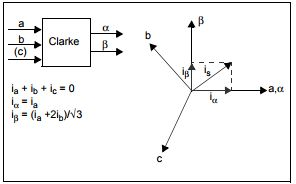
\includegraphics{imagenes/clarke.jpg}
	\caption{Transformada Clarke.}
\end{figure}
\FloatBarrier

\section{Transformada Park}
\begin{figure}[ht]
	\centering
	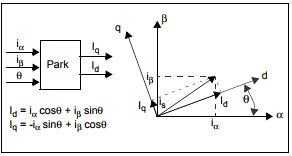
\includegraphics{imagenes/park.jpg}
	\caption{Transformada Park.}
\end{figure}
\FloatBarrier

\section{Controladores PI}
\subsection{Controlador de corriente}
\subsection{Controlador de velocidad}

\section{Transformada Park Inversa}
\begin{figure}[ht]
	\centering
	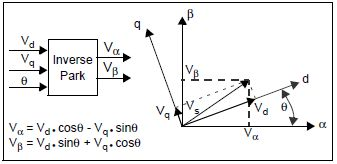
\includegraphics{imagenes/park_inv.jpg}
	\caption{Transformada Park Inversa.}
\end{figure}

\section{Modulacion de Espacio Vectorial}

\newpage
\section{Análisis de Proyectos Existentes}
\subsection{Odrive}

\begin{figure}[ht]
	\centering
	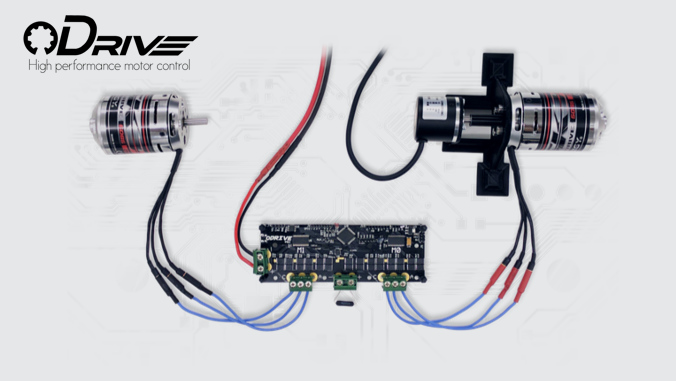
\includegraphics[scale=0.5]{imagenes/odrive_img.jpg}
	\caption{Odrive 3.6}
\end{figure}
\FloatBarrier

Odrive es uno de los controladores FOC comerciales mas populares para su uso en robotica por su gran versatilidad en sus ajsutes y un desempeño exelente para la mayoria de usos. internamente tiene opciones para control de torque, velocidad y posicion.

la version mas popular y generalemtne usada es Odrive 3.6, puede controlar 2 motores de forma simultanea, con hasta 56V y 70A continuos por motor,su codigo es open sourse, aun que solo hasta la vercion 3.5 mantuvo el open hardware, pero actualmente estas verciones estan descontinuadas, ya que el desarrollador esta trabajando en la vercion Odrive PRO.

aun que Odrive tiene un pequeño problema en su forma de operar internamente y es que su bucle se ejecuta a 8000hz, con un PWM de 24.000hz, esto principalemnte limita la electrica maxima que el motor puede controlar a un aproximado de 80.000 ERPM, lo que corresponde a 6 ciclos del bucle por cada giro electronico

\subsection{Vesc}
\begin{figure}[ht]
	\centering
	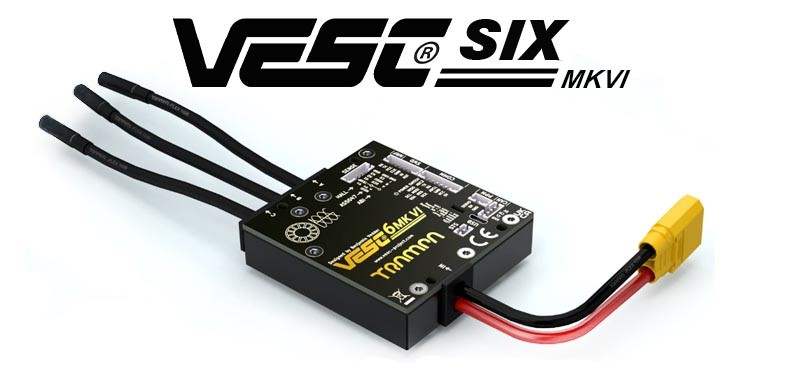
\includegraphics[scale=0.5]{imagenes/Vesc.jpg}
	\caption{Vesc 6}
\end{figure}
\FloatBarrier


\subsection{SimpleFOC}
\begin{figure}[ht]
	\centering
	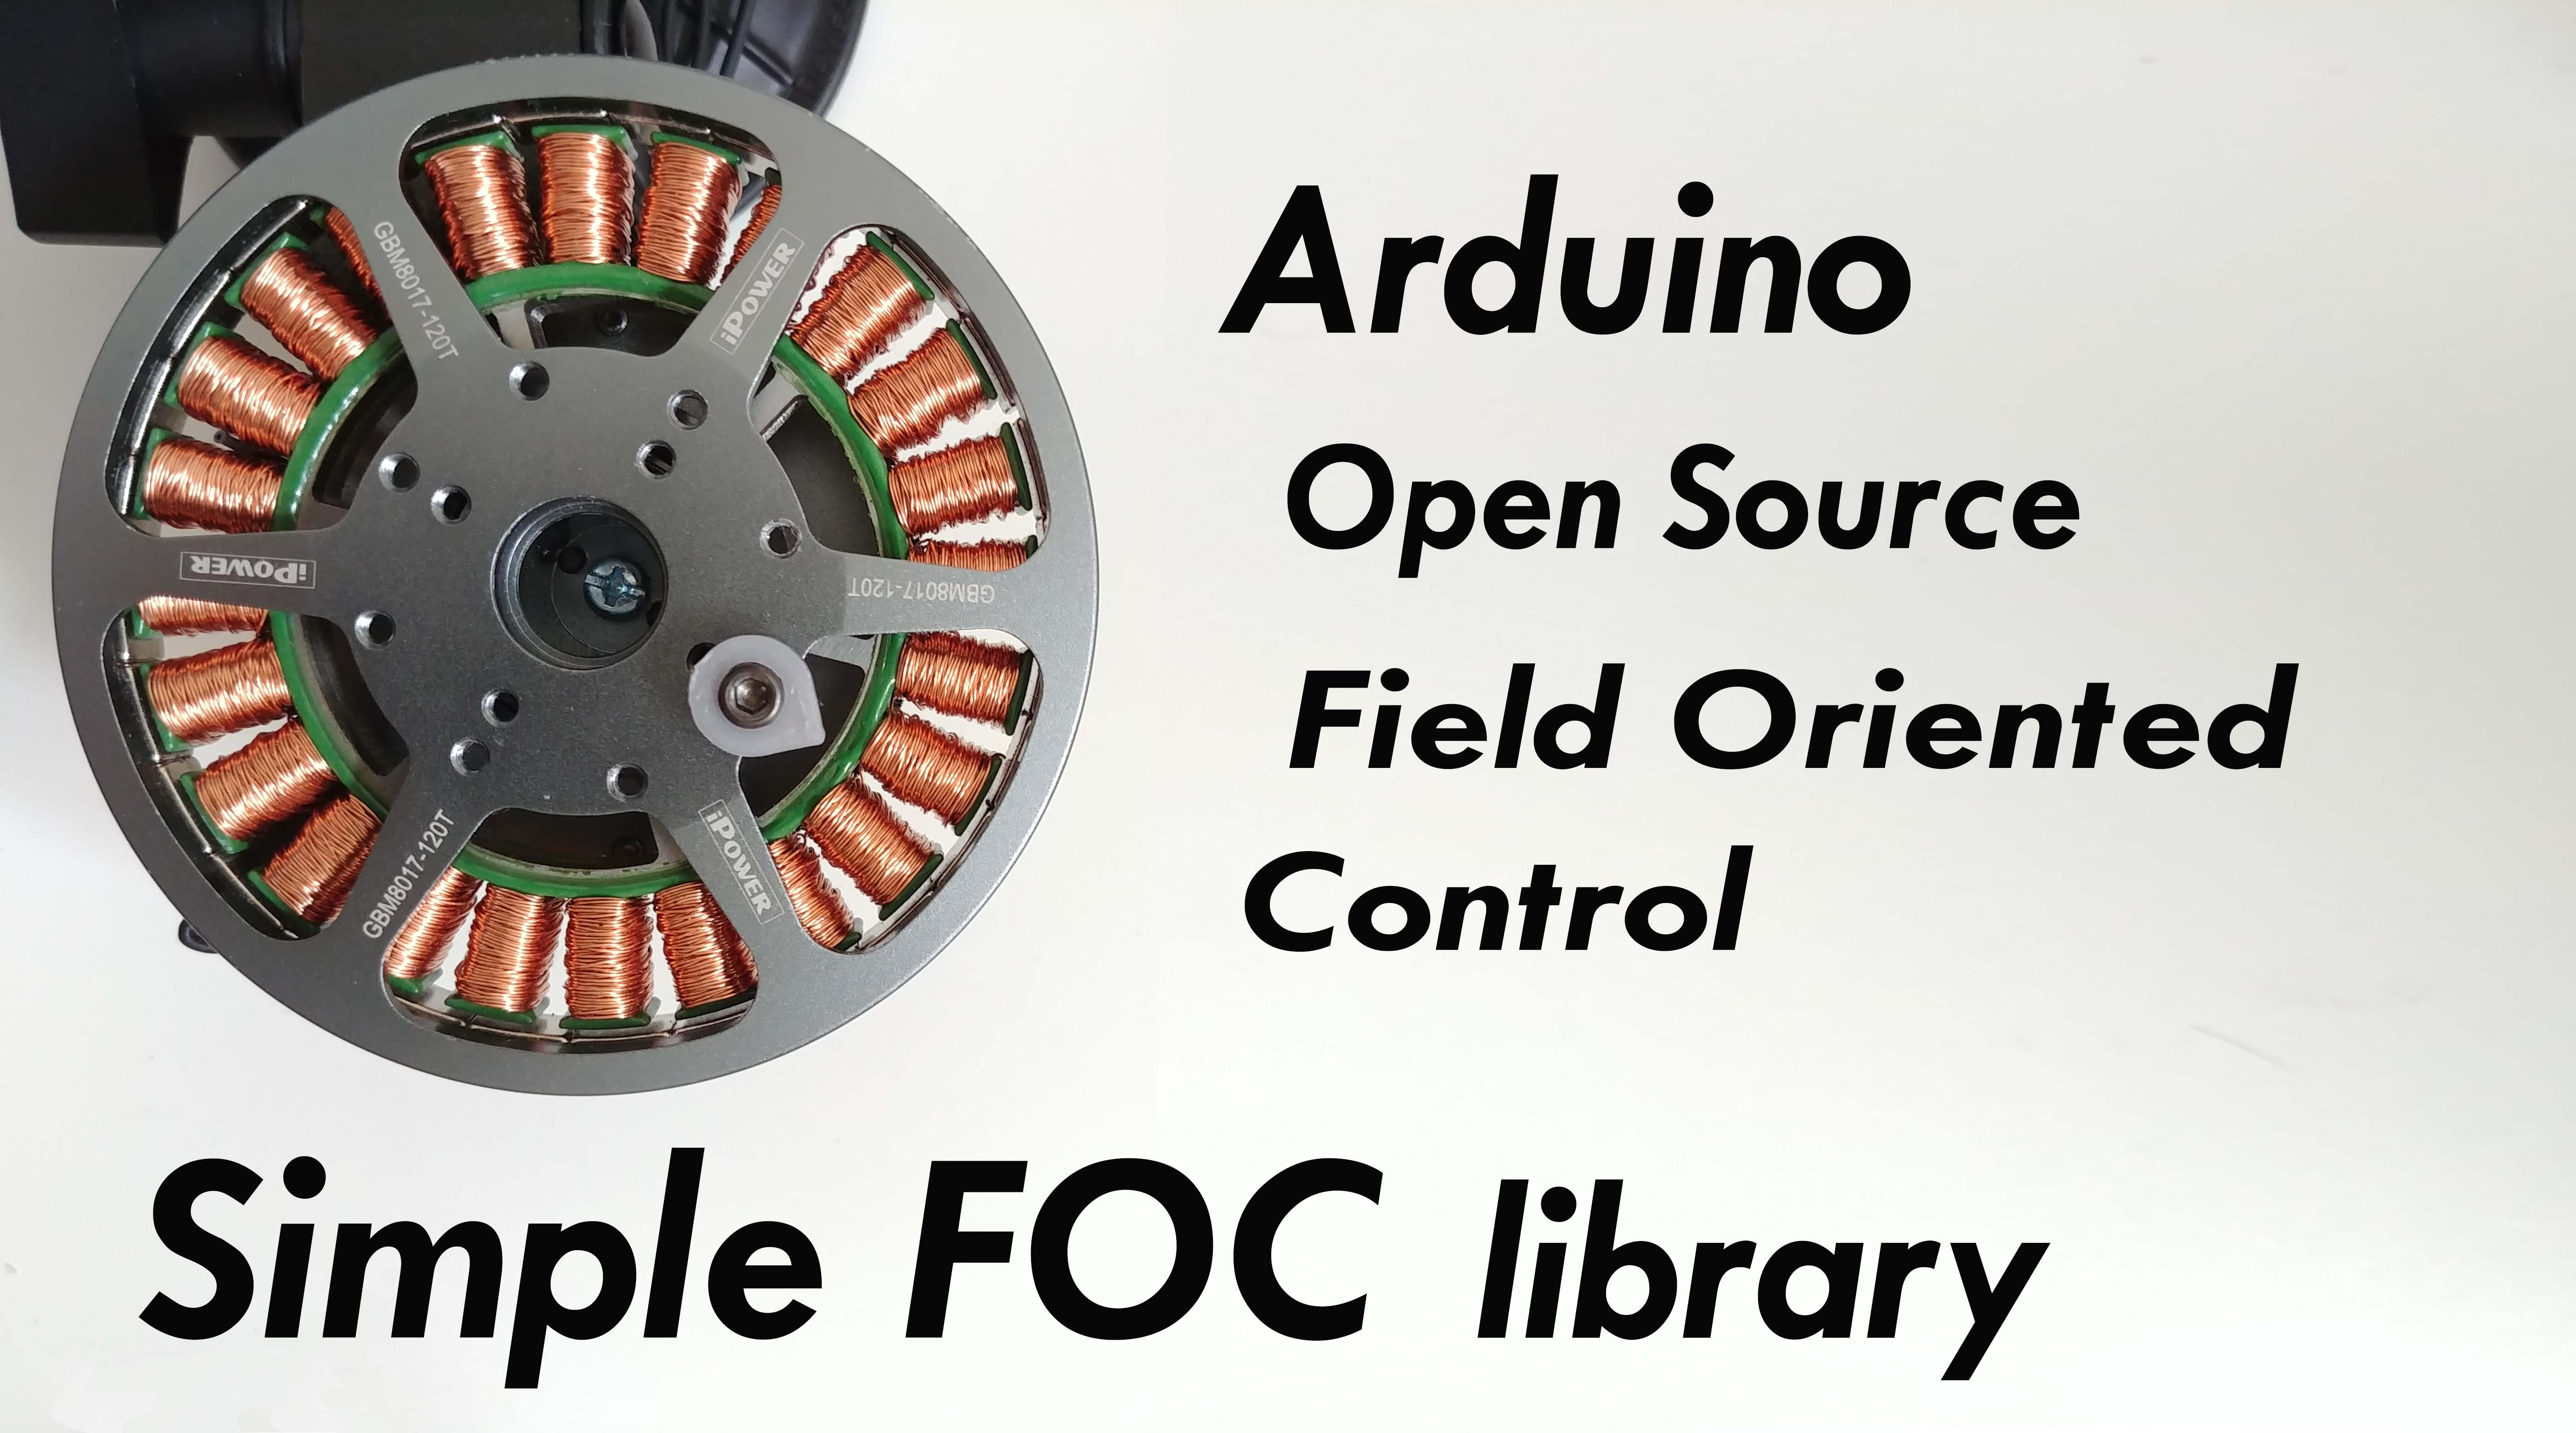
\includegraphics[scale=0.05]{imagenes/simpleFOC.jpeg}
	\caption{SimpleFOC}
\end{figure}
\FloatBarrier

SipleFOC \cite{Skuric_SimpleFOC_A_Field_2022} es una libreria Open Sourse para implementar controladores FOC utilizando arduino IDE o PlatformIO para compilar, este proyecto tiene como foco principa la facilidad de uso, siendo su principal uso en motores de tipo gimbal de baja potencia.

\newpage
\chapter{Diseño de Hardware para el Controlador FOC}
\section{Parametrización del Hardware para el Controlador FOC}
\subsection{Sensores de Corriente}
\subsection{Puente MOSFET}
\section{Implementación del Diseño Electrónico}

\newpage
\chapter{Configuración del STM32 con STM32CubeMX}

\newpage
\chapter{Implementación del Algoritmo de Control FOC}

\newpage
\chapter{Validación y Pruebas de Control FOC}
Este es un documento de ejemplo. Aquí hay una referencia a un libro \cite[p 200]{power_conv_00}.

Este es un documento de ejemplo. Aquí hay una referencia a un libro \cite[p 200]{AN2757_00}.

Este es un documento de ejemplo. Aquí hay una referencia a un libro \cite{odrive_SVM}.
\end{comment}

\begin{comment}
	\newpage
\subsection{Transformada de Clarke}
La transformada de Clarke es un procedimiento matemático que convierte un sistema trifásico de corrientes \(ABC\) en un sistema bifásico \(\alpha-\beta\). Esta transformación proyecta las corrientes trifásicas, referenciadas al estátor, en un sistema de coordenadas bidimensional estacionario con la misma referencia. \cite{AN1078}.

\begin{figure}[ht]
    \centering
    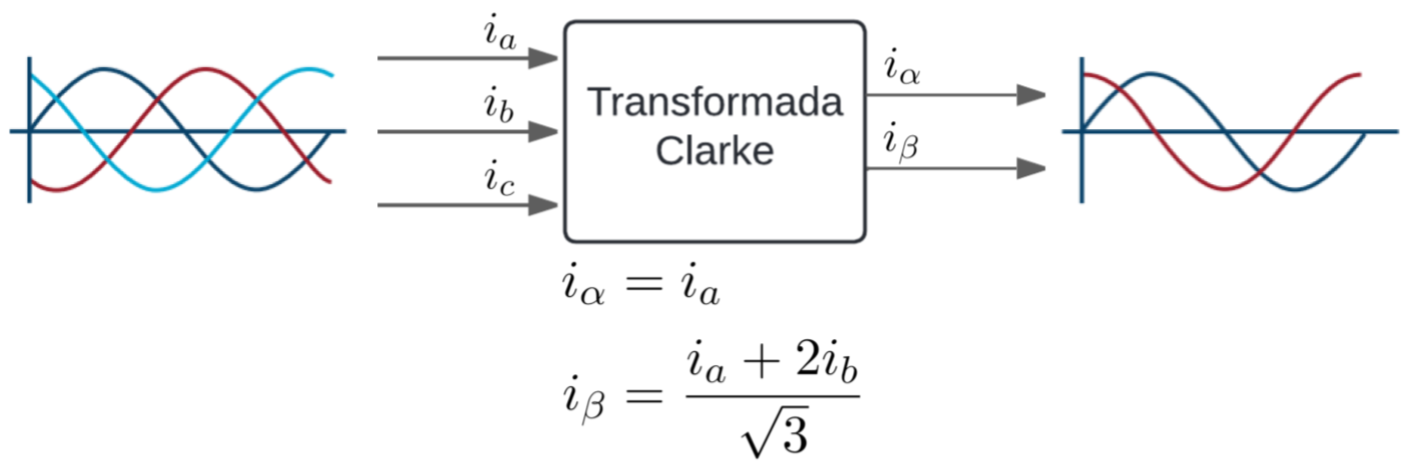
\includegraphics[width=0.5\textwidth]{imagenes/clarke.png}
    \caption{Transformada de Clarke \cite{AN1078}.}
    \label{fig:clarke_transform}
\end{figure}
\FloatBarrier

%Las expresiones utilizadas en la figura \ref{fig:clarke_transform} aprovechan la relación de los sistemas trifásicos equilibrados, donde se debe cumplir que \( I_a + I_b + I_c = 0 \), para simplificar el cálculo de los valores \(\alpha-\beta\). Esta simplificación se logra utilizando únicamente las corrientes \(I_a\) e \(I_b\), bajo el supuesto de que el sistema está equilibrado. En este caso, la corriente \(I_c\) puede ser estimada mediante la relación \(I_c = -(I_a + I_b)\), lo que permite reducir la cantidad de mediciones necesarias sin afectar el rendimiento del control.



\subsection{Transformada de Park}
La transformada Park convierte el sistema estacionario alpha-beta en un vector imaginario de dos dimensiones dq (directo y cuadratura) que se encuentra en un marco de referencia rotacional que gira de forma síncrona con el eje del motor. Esto permite convertir las corrientes alpha-beta, que varían en el tiempo, en los valores de corriente directa y cuadratura, que tienen un comportamiento continuo, simplificando así la medición de corriente en variables controlables \cite{AN1078}.
\begin{figure}[ht]
	\centering
	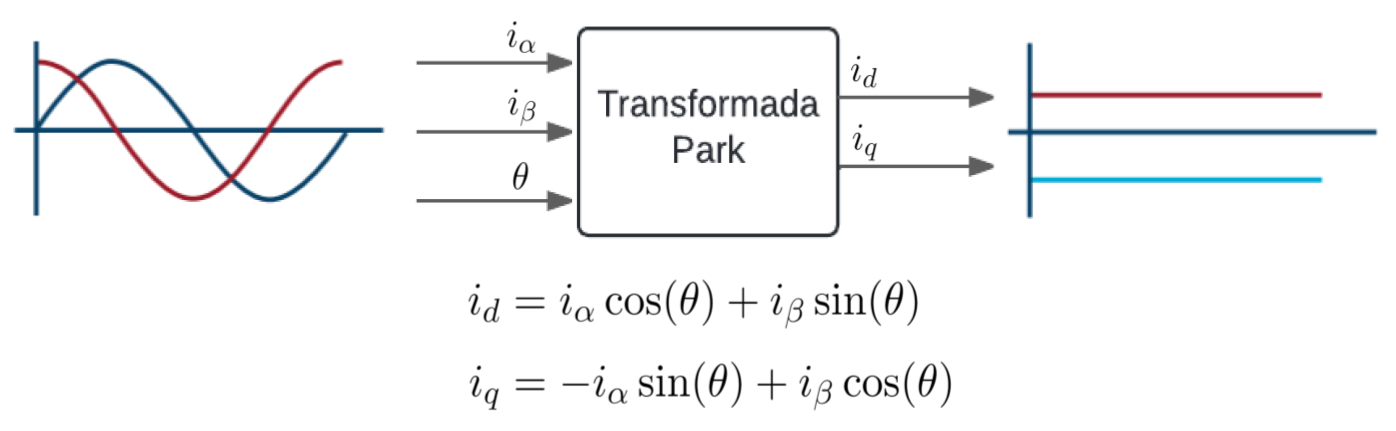
\includegraphics[width=0.5\textwidth]{imagenes/park.png}
	\caption{Transformada Park \cite{AN1078}.}
\end{figure}
\FloatBarrier

\subsection{Transformada inversa de Park}
También existe la transformada inversa de Park, que permite revertir esta transformación desde el marco de referencia rotacional y volver a las variables alpha-beta del marco de referencia estacionario \cite{AN1078}.

\begin{figure}[ht]
	\centering
	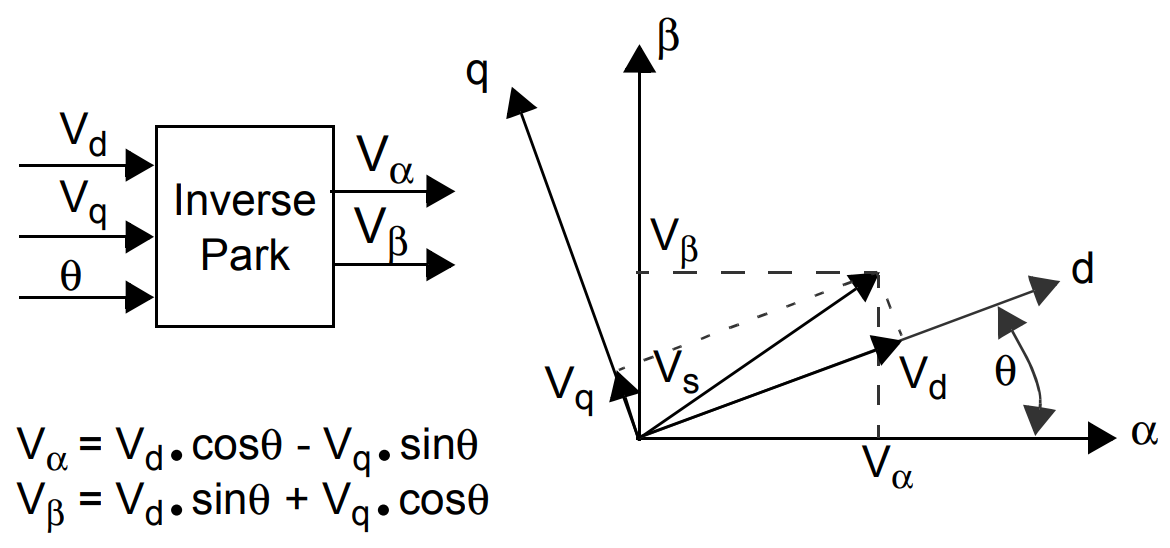
\includegraphics[width=0.5\textwidth]{imagenes/park_inv.png}
	\caption{Transformada Park Inversa \cite{AN1078}.}
\end{figure}
\FloatBarrier
\end{comment}

\end{document}
